\documentclass[11pt,a4wide]{article}
\usepackage{verbatim}
\usepackage{listings}
\usepackage{graphicx}
\usepackage{subcaption}
\usepackage{a4wide}
\usepackage{color}
\usepackage{amsmath}
\usepackage{amssymb}
\usepackage[dvips]{epsfig}
\usepackage[T1]{fontenc}
\usepackage{cite} % [2,3,4] --> [2--4]
\usepackage{shadow}
\usepackage{hyperref}
\usepackage{graphicx}
\usepackage[english]{babel}
\usepackage{float}
\usepackage{import}
\setcounter{tocdepth}{2}
\usepackage{listings}
\usepackage{color}
\usepackage{array}


\definecolor{blue}{rgb}{0,0,0.8}
\definecolor{mygray}{rgb}{0.5,0.5,0.5}
\definecolor{mymauve}{rgb}{0.58,0,0.82}

\lstdefinestyle{mystyle}
{ 
    backgroundcolor=\color{white},   
    commentstyle=\color{blue},
    keywordstyle=\color{magenta},
    numberstyle=\tiny\color{mygray},
    stringstyle=\color{mymauve},
    basicstyle=\footnotesize,
    frame=single,
    breakatwhitespace=false,         
    breaklines=true,                 
    captionpos=b,                    
    keepspaces=true,                 
    numbers=left,                    
    numbersep=5pt,                  
    showspaces=false,                
    showstringspaces=false,
    showtabs=false,                  
    tabsize=2, 
    stepnumber=2
}

\lstset{style=mystyle}


\begin{document}

\title{Solution to Newtonian Gravity problem with many bodies \break Computational Physics-Phy905 \break Project 3}
\author{Crispin Contreras}
\date{\today}
\maketitle


\begin{abstract}
This paper discusses the numerical solution to Newtonian Gravity with different planets in our solar system. Two methods were used to solve the problem one was the Verlet method and the other one was the Runge-Kutta to the fourth order (RK4). From these two methods we found tha the Verlet was more accurate and it was slightly faster in computational time. 
\end{abstract}



\section{Introduction}
I start by solving the the equations for Newtonian gravity. I begin with the simple Sun-Earth system and then move on to solve the Sun-Earth-Jupiter system with the Sun fixed and then the Sun-Earth-Jupiter with the Sun not fixed. Finally I model all the planets including Pluto. I used two different methods to solve this problem which are the Verlet and Runge-Kutta to the fourth order (RK4). These are just Taylor expansions and I discuss more about them in the Methods section. I test to see how stable the systems are by looking at different time steps and also increasing the time that the planets obit. Finally include my results and the conclusions that I arrived to. 

\section{Theory}
\subsection{Earth-Sun System}
I start with the Newtonian gravity which is given by $\ {\bf F} = - \frac{GM_1M_2}{r^2} {\bf \hat{r}}$. Here G is the gravitational constant, r is the distance between the bodies, and M represents the mass. I decided to work in Cartesian coordinates so I use 
\begin{equation}
\begin{split}
    {\bf \hat{r}} = cos(\theta){\bf \hat{x}} + sin(\theta){\bf \hat{y}}\\
    x=rcos(\theta), \hspace{0.3cm} y=rsin(\theta) \hspace{0.3cm} r = \sqrt{x^2 + y^2}
\end{split} 
\end{equation}
Where $\ \theta$ is just the polar angle. Now using equation (1) I break the equation for gravitation into Cartesian coordinates 
\begin{equation}
\begin{split}
	F_x = -\frac{GM_1M_2}{r^3}x \\
	F_y = -\frac{GM_1M_2}{r^3}y 
\end{split}
\end{equation}
With equation (2) now I can start setting up the equations of motions for the planets. I start with the Earth-Sun system where I treat the Sun as stationary so I use it as the origin. I start with the equations of motion, for simplicity I will only do the x coordinate since the only thing that changes in the others is the coordinate itself.  
\[
	M_{Earth}\frac{d^2x}{dt^2} = -\frac{GM_{Earth}M_{Sun}}{r^3}x
\]
I will simplify this equation further by introducing a new set of units for the G and mass. The Earth's orbit around the sun is almost circular around the Sun so for this type of motion the force is given by 
\[
	F =\frac{M_{Earth}v^2}{r}=\frac{GM_{Sun}M_{Earth}}{r^2}
\]
from this equation we can get rid of the gravitational constant G and mass of the sun to replace it by 
\begin{equation}
	v^2r=GM_{Sun}=4\pi^2 (\frac{AU^3}{yr^2})
\end{equation}
with this transformation now we can use the astronomical units (AU) for length and year (yr) for time. The mass of the Sun is then one. Now the equation of motion for the earth reads 
\begin{equation}
\begin{split}
	F_x = \frac{d^2v_x}{dt^2} = -\frac{4\pi^2}{r^3}x \\
	\frac{dx}{dt}=v_x
\end{split}
\end{equation}
The equation for the y coordinate is the same except the x is replace by y. 
\subsection{Three Body Problem}
I start with a simplified version of the three body problem. In this case I model the Sun, Earth, and Jupiter but I will keep the Sun fixed. For the Earth the only thing that changes now is that it feel the force from Jupiter. The force now reads
\begin{equation}
	F_x^{Earth}= \frac{dv_{x_E}}{dt} =-\frac{4\pi^2}{r_{ES}^3}x_E - \frac{4\pi^2(M_{Jupiter}/M_{Sun})}{r_{EJ}^3}(x_E -x_J)
\end{equation}
where now include the coordinates for Jupiter, $\ r_{EJ}$ is the distance between the Earth and Jupiter, and $\ r_{ES}$ is the distance between the Earth and the Sun. Here $\ x_J$ is the position of Jupiter and $\ x_E$ is the position of the Earth and M represents the mass of the bodies. The same equation for (5) is obtained for y  except the x is replace by either y. $\ r_{EJ}$ is given by 
\[
	r_{EJ}=\sqrt{(x_E -x_J)^2+(y_E -y_J)^2+}
\]
For Jupiter I obtain the equation 
\begin{equation}
	F_x^{Jupiter}= \frac{dv_{x_J}}{dt} =-\frac{4\pi^2}{r_{JS}^3}x_J - \frac{4\pi^2(M_{Earth}/M_{Sun})}{r_{EJ}^3}(x_J -x_E)
\end{equation}
here $\ r_{JS}$ is the distance between Jupiter and the Sun, in order to get the y coordinate I just replace x by y.  

Now to do the full three body problem I will allow the Sun to move instead of being fixed. This means that the origin of the system is now the center of mass of the three bodies. I give the equation for the Sun 
\begin{equation}
	F_x^{Sun}= \frac{dv_{x_S}}{dt} =-\frac{4\pi^2(M_{Jupiter}/M_{Sun})}{r_{JS}^3}(x_S- x_J) - \frac{4\pi^2(M_{Earth}/M_{Sun})}{r_{SE}^3}(x_S -x_E)
\end{equation}
for equations (5) and (6) the only thing that gets modified is the term $\ x_J$ which goes to $\ (x_J -x_S)$ and $\ x_E$ which goes to $\ (x_E -x_S)$, the same thing occurs for the y variable. With equations (5),(6),and (7) now I can solve the three body problem in two dimensions. 
	
Finally to model the all the planets of the solar system and Pluto, I keep the sun fixed for simplicity. In general the equation is given by 
\begin{equation}
	F_x^j = -\frac{4\pi^2}{r_{jS}^3}(x_j-x_S) -4\pi^2\sum_{ i=1,j\neq i}^9{\frac{M_i/M_{Sun}}{r_{ji}^3}(x_j-x_i)}
\end{equation} 
here j and i can take on the values $\ j,i =1,2,3...9$ and they represent how far the planet is from the Sun. For example Mercury will be 1, Venus 2, and so on. Now that I have all the equations setup I can move on to describe the methods. 



\section{Methods}
Two methods were implemented to solve the equations above. I used the Verlet method which has an accuracy of $\ h^5$. I also used the Runge-Kutta 4 which is more precise than the Verlet but has more floating point operations. The basic idea behind these two methods is to use a Taylor expansion and for each one have a different truncation. I take much of the derivations from [1]. 
\subsection{Velocity Verlet Method}
In order to derive the algorithm for the Verlet I will start by using Newton's second law  in one dimension which reads
\[
	m\frac{d^2x}{dt^2} = F(x,t) 
\]
this can be rewritten in terms of couple equation such that 
\[
	\frac{dx}{dt}=v_x  \hspace{0.3cm} and \hspace{0.3cm} \frac{dv}{dt}=F(x,t)/m=a(x,t)
\]
I also define the time step which I'm going to use which is $\ h=\frac{t_f -t_i}{n}$, here n is the step size. We want h to be small so we can perform a taylor expansion such that 
\[
	x(t+h)= x(t)+hx'(t) + \frac{h^2}{2}x''(t) + \mathcal{O}(h^3)
\]
now I will introduce the notation for discretized equation in terms of h. 
\begin{equation}
	x(t_i \pm h)=x_{i\pm 1} \hspace{0.3cm} x_i=x(t_i)
\end{equation}
here i can range from 0, which is the initial time, to n. Now I will do the expansion in this discrtetized for the position and velocity 
\begin{equation}
\begin{split}
	x_{i+1} = x_i + hx'_i + \frac{h^2}{2}x''_i + \mathcal{O}(h^3) \\
	v_{i+1} = v_i + hv'_i + \frac{h^2}{2}v''_i + \mathcal{O}(h^3)
\end{split}
\end{equation}
from Newton's second law then we have 
\[
	v'_i = \frac{d^2x_i}{dt^2}=F(x_i,t_i)/m
\]
From equation (10) we see that for the position we know all the variable up to the second order but for velocity we don't v''. In order to address this problem we have to make another approximation given by 
\[
	v'_{i+1} = v'_i + hv''_i + \mathcal{O}(h^2)
\]
with this approximation I obtain a value for $\ v''_i$ which is $\ v''_i \approx v'_{i+1} - v'_i$. Now I know the value of v'' in terms of v', I substitute this into the velocity equation in (10) which give me 
\begin{equation}
	v_{i+1} = v_i + \frac{h}{2}\left(v'_{i+1} + v'_i \right) + \mathcal{O}(h^3)
\end{equation}
with equation (10) and (11) we are now able to solve the problem. Equations (10) and (11) transform to 
\begin{equation}
\begin{split}
	x_{i+1} = x_i + hv_i - \frac{h^2}{2}\frac{4\pi^2}{r_i^3}x_i \\
	v_{i+1} = v_i -\frac{h}{2}\left(\frac{4\pi^2}{r_{i+1}^3}x_{i+1} + \frac{4\pi^2}{r_i^2}x_i\right)
\end{split}
\end{equation}
Equation (12) is used for the calculation of the Earth-Sun system and it's only for the x coordinate. Using this algorithm we see that the order of precision is $\ \mathcal{O}(h^3)$. The same is done for the y coordinate and for the other systems this same algorithm is used but with different forces. This is shown in listing 1. 


\lstinputlisting[language =C++,firstline=25, lastline=136, caption = This shows how velocity Verlet method is implemented.]{"/home/quetzalcoatl/Computational_Physics_work/Project3/Code/solver.cpp"}

\subsection{Runge-Kutta 4 method}
The idea behind the Runge-Kutta method is similar to the velocity verlet methods in that again we use a Taylor approximation of the function we want to find. But it's is more accurate since there are several more approximations made than in the velocity Verlet. I start with the a general function 
\[
	\frac{dy}{dt} = f(t,y)
\]
this type of function can be solve by integrating and the results with a discretized function as in the Verlet method is 
\[
	y_{i+1} = y_i + \int_{t_i}^{t_{i+1}}f(t,y)dt
\]
the next critical approximation comes from the integral part of the equation. To approximate the integral we use Simpson's rule which is given by 
\[
	\int_{t_i}^{t_{i+1}}f(t,y)dt \approx \frac{h}{6}\left[ f(t_i,y_i) + 4f(t_{i+1/2},y_{i+1/2}) + f(t_{i+1},y_{i+1}) \right]
\]
In this method we split the midpoint evaluation into two which gives us 
\[
	\int_{t_i}^{t_{i+1}}f(t,y)dt \approx \frac{h}{6}\left[ f(t_i,y_i) + 2f(t_{i+1/2},y_{i+1/2})+ 2f(t_{i+1/2},y_{i+1/2}) + f(t_{i+1},y_{i+1}) \right]
\]
To solve for the values of f at different at different times we us the predictor corrector methods which consists of finding the slope at the function $\ t_i$ which is given by $\ k_1 = f(t_i, y_i)$. Then make a prediction for the solution using Euler's method and use this prediction to compute a new slope at this time. After finding the prediction for the slopes then we average the results. In the Runge-Kutta method to the fourth order (RK4) we do this four times. To help us visualize this better I will use figure 1 which shows where I will be taking the approximations. 
 
	We begin by looking at time $\ t_i$ and finding the slope here, the slope here is given by $\ k_1=hf(t_i,y_i)$. The next time step is then $\ t_{i+1/2}$. In this time step we will make two prediction for the slope which will be approximated using Euler's method. For the predictions we have
\begin{equation}
	y_{(i+1/2),Prediciton 1} = y_i + \frac{h}{2}\frac{dy}{dt} = y_i + \frac{h}{2}f(t_i,y_i) = y_i + \frac{k_1}{2} \\
\end{equation}
with equation (13) I can now find the second estimate for slope which is given by 
\[
	k_2 =f(t_{i+1/2},y_{(i+1/2),Prediciton 1})=f(t_{i+1/2},y_i + \frac{k_1}{2})
\]
we make another prediction to find the next slope this is then 
\begin{equation}
	y_{(i+1/2),Prediciton 2} = y_i + \frac{h}{2}\frac{dy}{dt} = y_i + \frac{h}{2}f(t_{i+1/2},y_{(i+1/2),Prediciton 1}) = y_i + 	\frac{k_2}{2}
\end{equation}
and for the next slope we have
\[
	k_3 = hf(t_{i+1/2},y_{(i+1/2),Prediciton 2}) = f(t_{i+1/2},y_i +\frac{k_2}{2} )
\]
and finally for the last slope we have 
\[
	k_4 = hf(t_{i+1}, y_{(i+1),Prediction 3} = f(t_{i+1}, y_i + k_3)
\]
here we use the approximation for Prediction 3
\[
	y_{i+1} = y_i + hf(t_{i+1/2},y_{i+1/2})
\]
which is know as the midpoint formula. Now we have all the values the slopes and we can use Simpson's rule above to arrive at the equation 
\begin{equation}
	y_{i+1} = y_i + \frac{h}{6}\left[k_1 + 2k_2 + 2k_3 + k_4 \right] 
\end{equation}
with equation (16) we can now implement the RK4 method. 

\begin{figure}[H] 
\centering
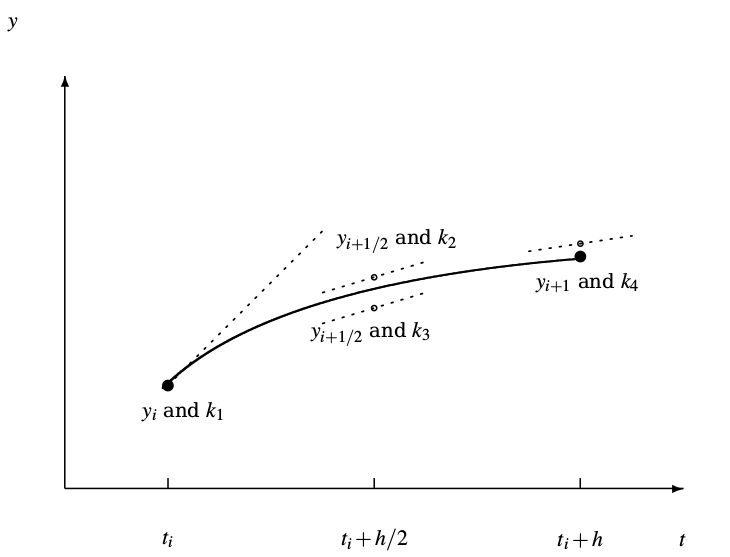
\includegraphics[width=100mm]{RK4.png}
\caption{ Plot of a general function and the differernt approximations taken in order to find the different slopes [1] \label{overflow}}
\end{figure}
	
	Equation (16) changes with the coordinate your using and also the force that each planet feels so this has to be modified also. In our case we start with the equation for velocity which means we have to use the method twice. This means we find the k for the positions and the velocities. The way this algorithm is implimented is shown in the following listing.
	
\lstinputlisting[language =C++,firstline=148, lastline=370, caption = This shows how velocity RK4 method is implemented.]{"/home/quetzalcoatl/Computational_Physics_work/Project3/Code/solver.cpp"}

%*****************************************************************************************************************************
% Resutls section 
%******************************************************************************************************************************
\section{Results}

	Here we begin to discuss the results of the program. We start by discussing the stability of both the RK4 and the Velocity Verlet method. To see whether it's stable we looked at the total energy and the angular momentum which should be conserved. Additionally we looked at their orbits and how much they varied. In the Discussion section I will only look closely at the Earth and Sun System which was enough to verify the program was working correctly. I next get the results for the Earth-Jupiter system and using the results from the Earth-Sun system I figure out the stability. In the Earth Jupiter system I look at how Jupiter effects Earth's orbit.First by looking at the original mass of Jupiter, then at 10 times of its original mass, and finally at 1000 times its original mass. Finally I look at the entire solar system, for this I use JPL's solar system data. To solve this problem I used two different classes one which was the plant and the solver. The planet class contained all the information for the planets and the solver contained the RK4 and the Velocity Verlet. This is given in the Code Attachment section. 


%****************************************************************************************************************
% This part goes in to the Discussion
%****************************************************************************************************************

\section{Discussion}
\subsection{Earth Bound and Unbounded}

	Here I will look at the stability of the Earth and Sun system, computational speed, and also vary the initial speed of the Earth to see where the escape velocity occurs. From our results that the Velocity Verlet algorithm is the fastest on some ocassions and also it has less error. This of course was expected since the relative error in the Velocity Verlet is $\ h^4$ and for the global error in the RK4 this is just $\ h^3$. 
\begin{table}[H]
\centering
\label{my-label}
\begin{tabular}{| m{3cm} | m{3cm} | m{3cm} |}
 \cline{1-3}
 n&  Verlet Time [s]&  RK4 Time[s]\\ \cline{1-3}
 100&  0.001393& 0.001517\\ \cline{1-3}
 200&  0.001385& 0.0.003136\\ \cline{1-3}
 500&  0.007372& 0.06474\\ \cline{1-3}
 1000&  0.014618& 0.014609\\ \cline{1-3}
 2000&  0.02704& 0.027904\\ \cline{1-3}
 5000&  0.068593& 0.06544\\ \cline{1-3}
 10000&  0.123608& 0.128265\\ \cline{1-3}
\end{tabular}
\caption{This table gives the number of grid points used n, and the computational time. From here we see that the Velocity Verlet method is faster most of the time. }
\end{table}

	For the Earth to have a circular we found that the speed had to be $\ 2\pi (AU/yr)$ at radius 1 AU. At this same distance we kept increasing the speed to find were the escape velocity. The escape velocity for this configuration is $\ 2\sqrt{2}\pi (Au/yr)$. As we get close to this speed the orbit of the Earth reaches an ellipse and the finally it escapes. We can tell if the Earth is bounded by the potential if the total energy, which is the sum of the kinetic and potential, is positive. 

%**************************************************************
% Radius 
%**************************************************************

\begin{figure}[H]
\begin{subfigure}[b]{0.5\linewidth}
    \centering
    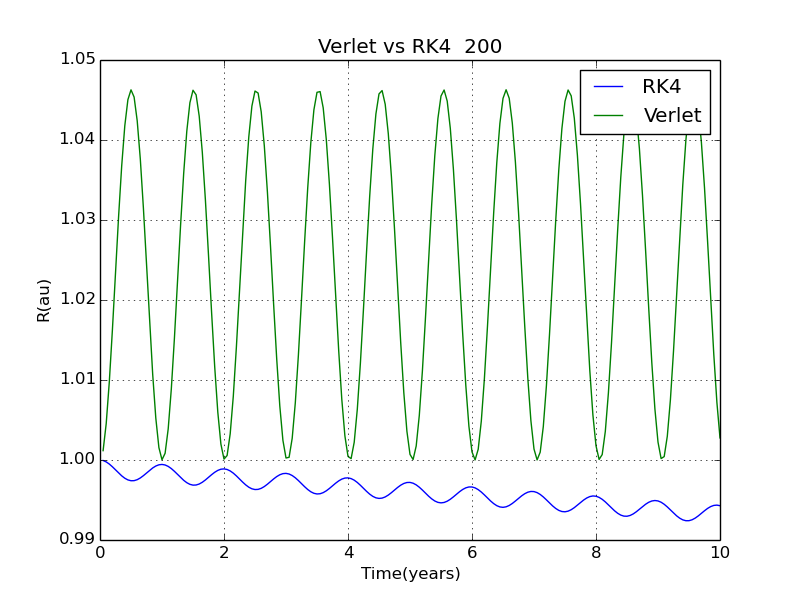
\includegraphics[width=70mm]{200.png}
    \caption{Value of radius for n=200} 
    \label{fig7:a} 
    \vspace{4ex}
\end{subfigure}%%
\begin{subfigure}[b]{0.5\linewidth}
    \centering
    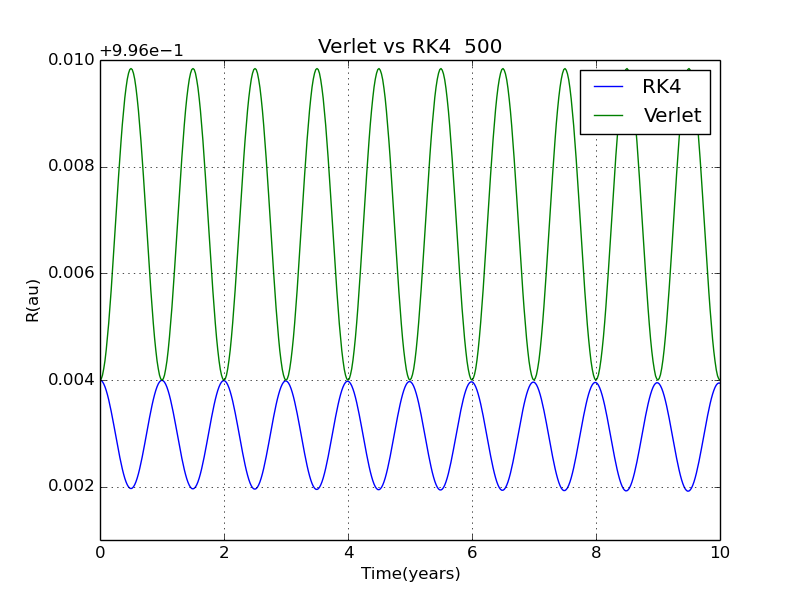
\includegraphics[width=70mm]{500.png}
    \caption{Value of radius for n=500} 
    \label{fig7:b} 
    \vspace{4ex}
\end{subfigure}
\begin{subfigure}[b]{0.5\linewidth}
    \centering
    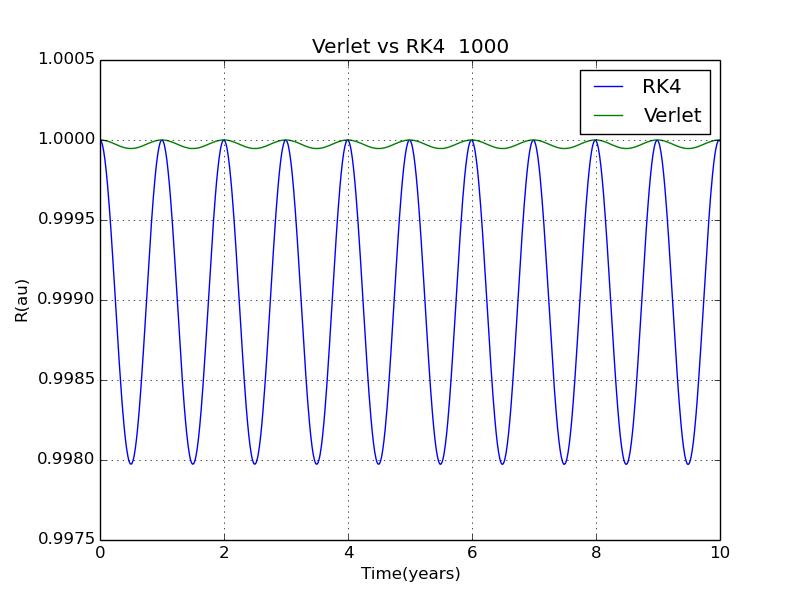
\includegraphics[width=70mm]{1000.png}
    \caption{Value of radius for n=1000} 
    \label{fig7:c} 
    \vspace{4ex}
\end{subfigure}%%
\begin{subfigure}[b]{0.5\linewidth}
    \centering
    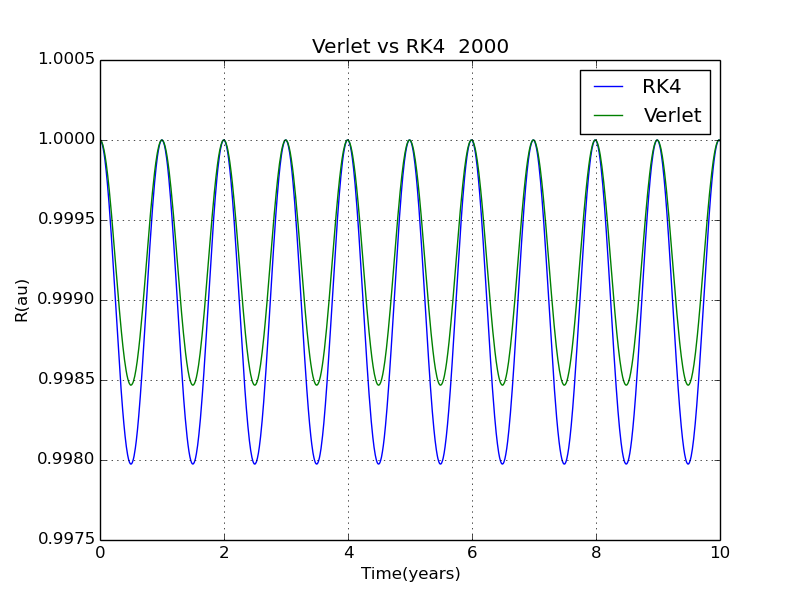
\includegraphics[width=70mm]{2000.png}
    \caption{Value of radius for n=2000} 
    \label{fig7:d} 
    \vspace{4ex}
\end{subfigure}
\caption{This shows the values of the radius for different values of n. From (a) and (b) we can see that the RK4 is a bit more stable than the Velocity Verlet. But as the value of n goes up the Velocity Verlet reaches stability at about n=1000. After this the Velocity Verlet is unstable and behaves similarly to RK4. From this we can gather that the Velocity Verlet is much more accurate.}
\end{figure}

%*******************************************************************
% Total Energy 
%*******************************************************************

\begin{figure}[H]
\begin{subfigure}[b]{0.5\linewidth}
    \centering
    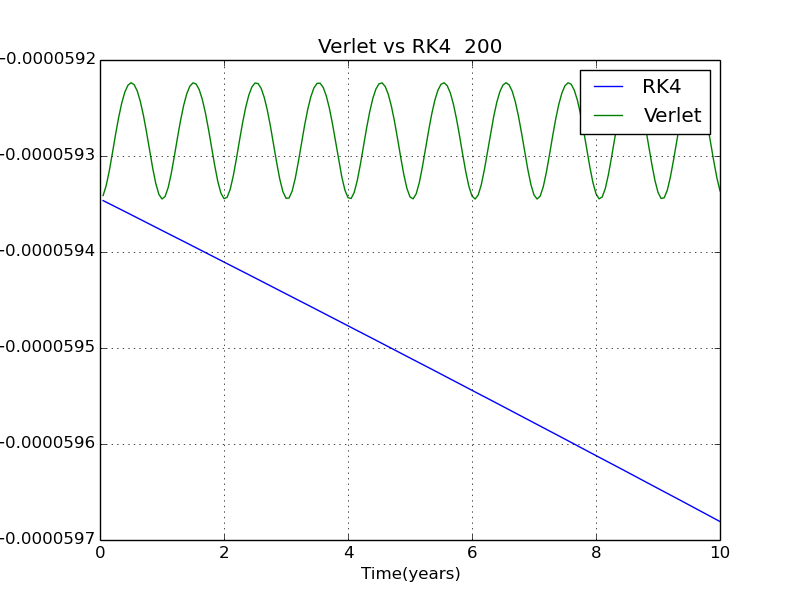
\includegraphics[width=70mm]{E200.png}
    \caption{Total Energy $\ (Au/yr)^2$ for n=200} 
    \label{fig7:a} 
    \vspace{4ex}
\end{subfigure}%%
\begin{subfigure}[b]{0.5\linewidth}
    \centering
    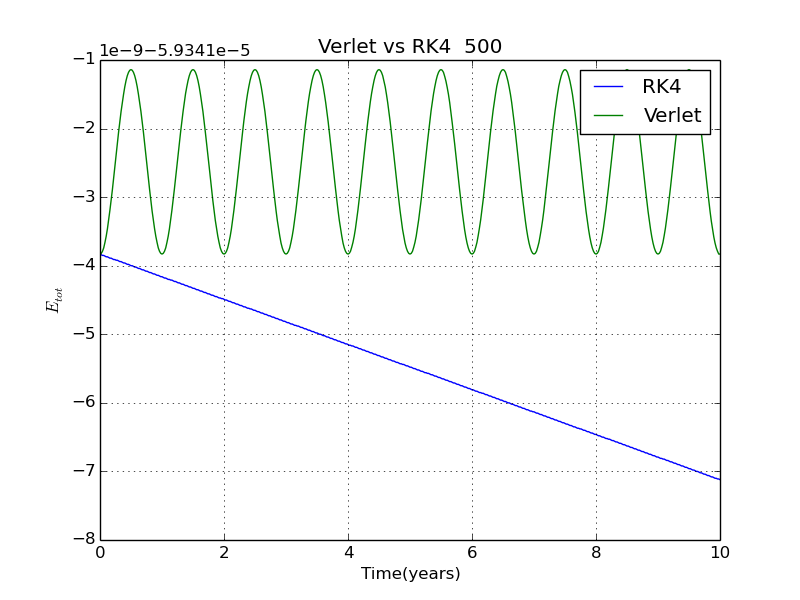
\includegraphics[width=70mm]{E500.png}
    \caption{Total Energy $\ (Au/yr)^2$ for n=500} 
    \label{fig7:b} 
    \vspace{4ex}
\end{subfigure}
\begin{subfigure}[b]{0.5\linewidth}
    \centering
    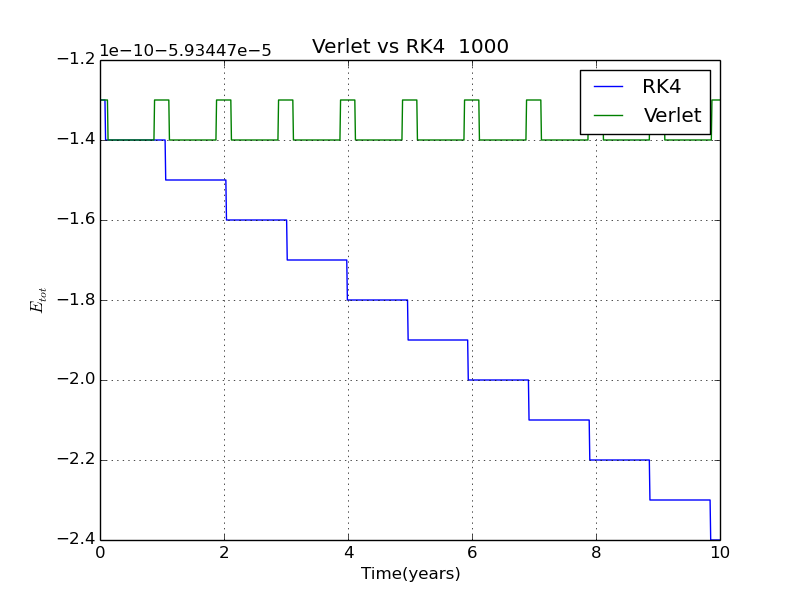
\includegraphics[width=70mm]{EE3.png}
    \caption{Total Energy $\ (Au/yr)^2$ for n=1000} 
    \label{fig7:c} 
    \vspace{4ex}
\end{subfigure}%%
\caption{This shows the Values of the total energy for different values of n. Again we can clearly see that the Velocity Verlet method is more accurate.}
\end{figure}

%**************************************************************
% Bound and Unbounded
%**************************************************************
\begin{figure}[H]
\begin{subfigure}[b]{0.5\linewidth}
    \centering
    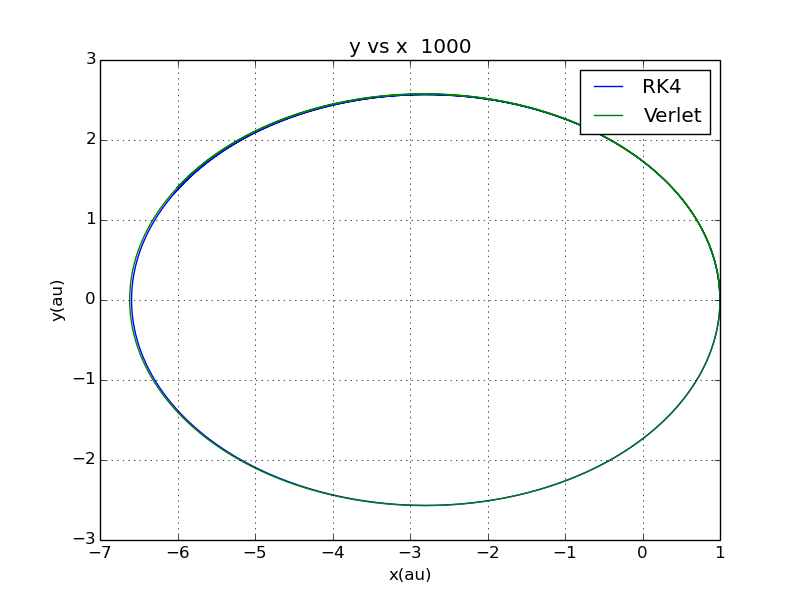
\includegraphics[width=70mm]{Ellipse.png}
    \caption{Position of the Earth in x and y} 
    \label{fig7:a} 
    \vspace{4ex}
\end{subfigure}%%
\begin{subfigure}[b]{0.5\linewidth}
    \centering
    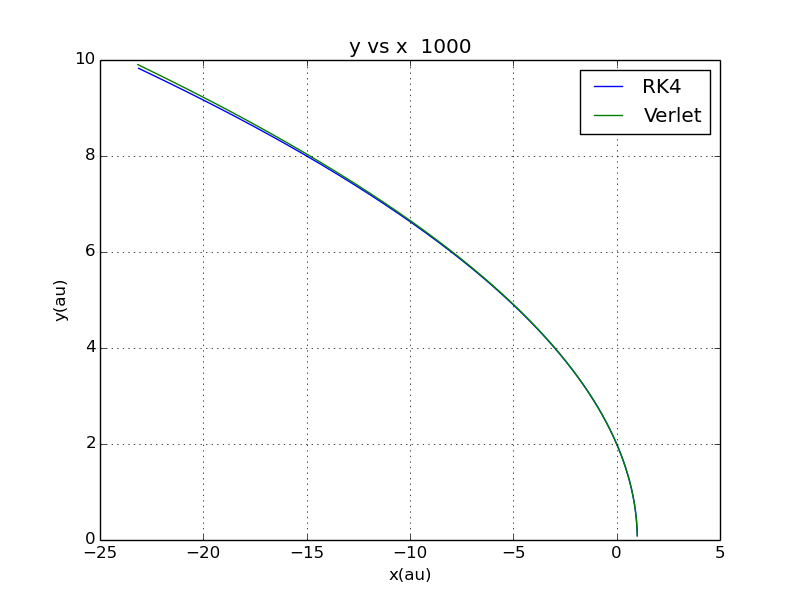
\includegraphics[width=70mm]{Escape.png}
    \caption{Posiion of the Earth in x and y} 
    \label{fig7:b} 
    \vspace{4ex}
\end{subfigure}
\begin{subfigure}[b]{0.5\linewidth}
    \centering
    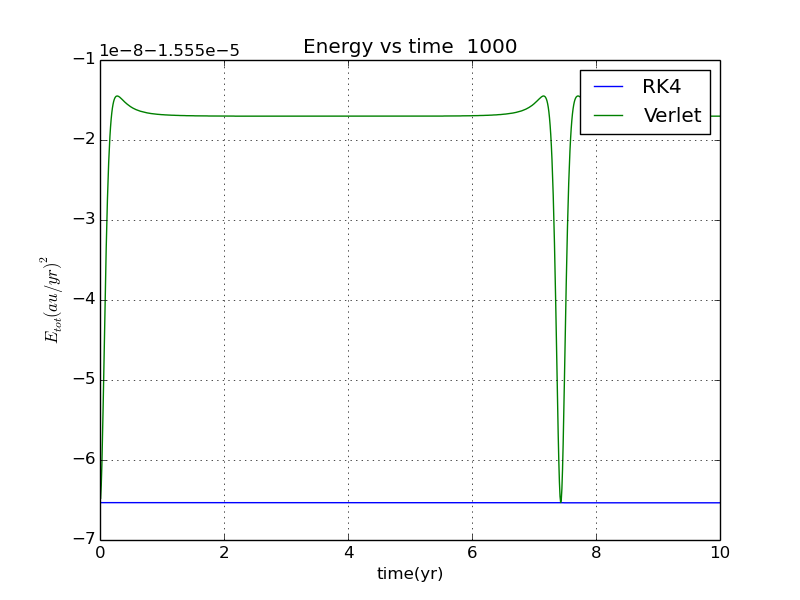
\includegraphics[width=70mm]{EEllipse.png}
    \caption{Total Energy $\ (Au/yr)^2$ for n=5000} 
    \label{fig7:c} 
    \vspace{4ex}
\end{subfigure}%%
\begin{subfigure}[b]{0.5\linewidth}
    \centering
    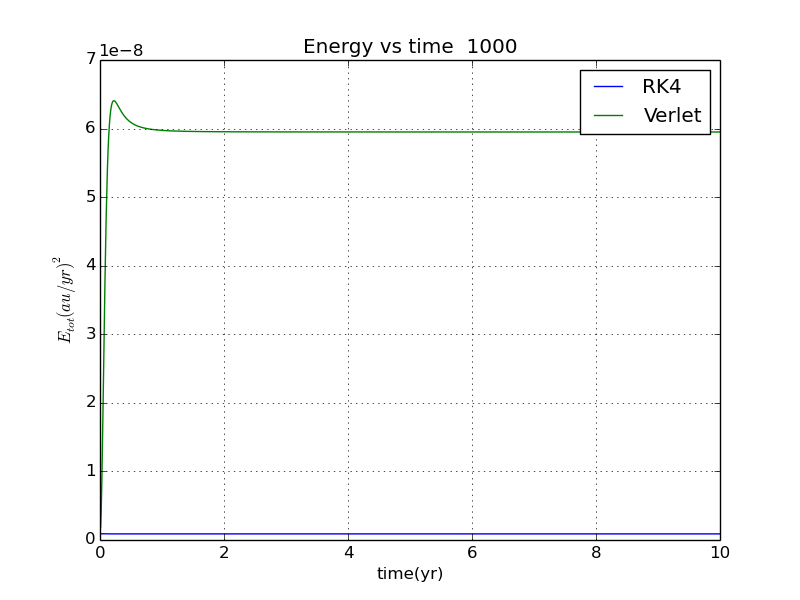
\includegraphics[width=70mm]{EEscape.png}
    \caption{Total Energy $\ (Au/yr)^2$ for n=5000} 
    \label{fig7:d} 
    \vspace{4ex}
\end{subfigure}
\caption{(a) and (b) are plot of the x and y coordinates of the Earth when the velocity will approach the escape velocity. (c) and (d) show their respective energies. This was done with n=5000.}
\end{figure}

\subsection{Earth Jupiter System}

%**********************************************************************************
% Position of various configuration of mass of Jupiter
%**********************************************************************************
\begin{figure}[H]
\begin{subfigure}[b]{0.5\linewidth}
    \centering
    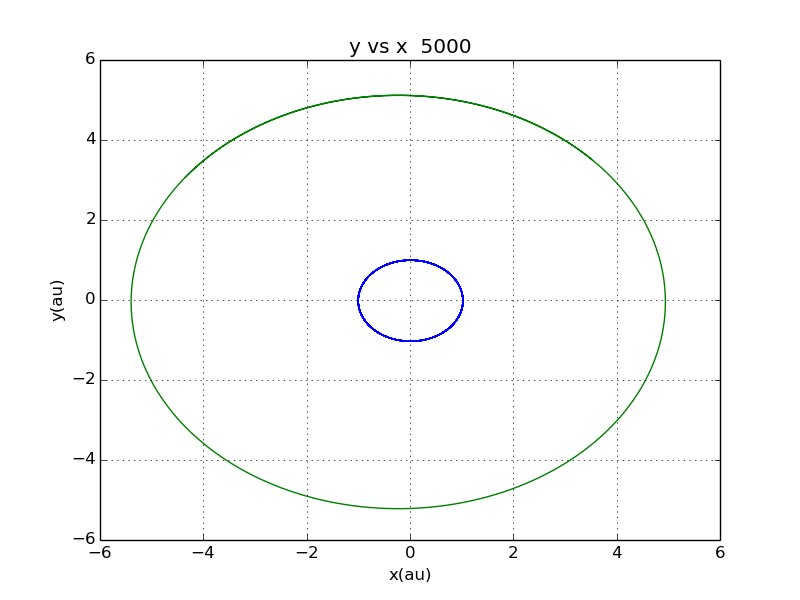
\includegraphics[width=70mm]{EJ.png}
    \caption{Jupiter's original mass} 
    \label{fig7:a} 
    \vspace{4ex}
\end{subfigure}%%
\begin{subfigure}[b]{0.5\linewidth}
    \centering
    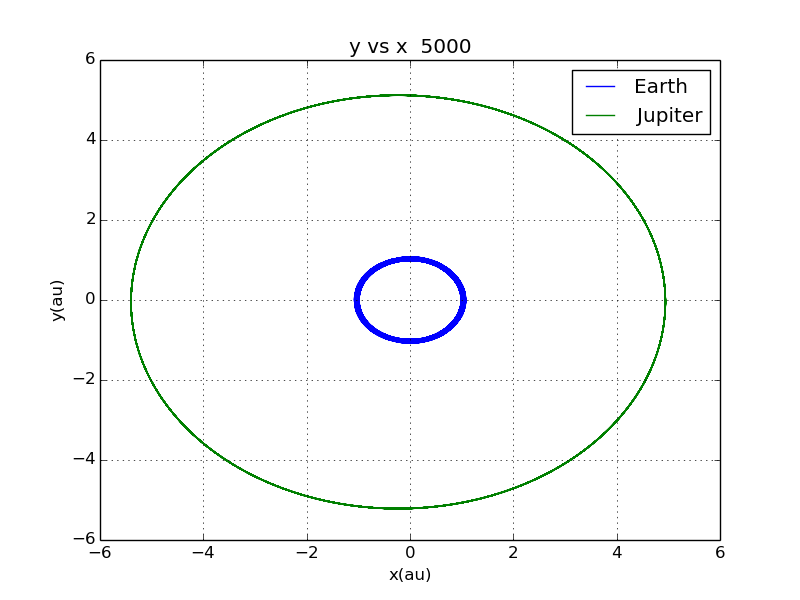
\includegraphics[width=70mm]{EJ_10V.png}
    \caption{Jupiter with 10 the original mass} 
    \label{fig7:b} 
    \vspace{4ex}
\end{subfigure}
\begin{subfigure}[b]{0.5\linewidth}
    \centering
    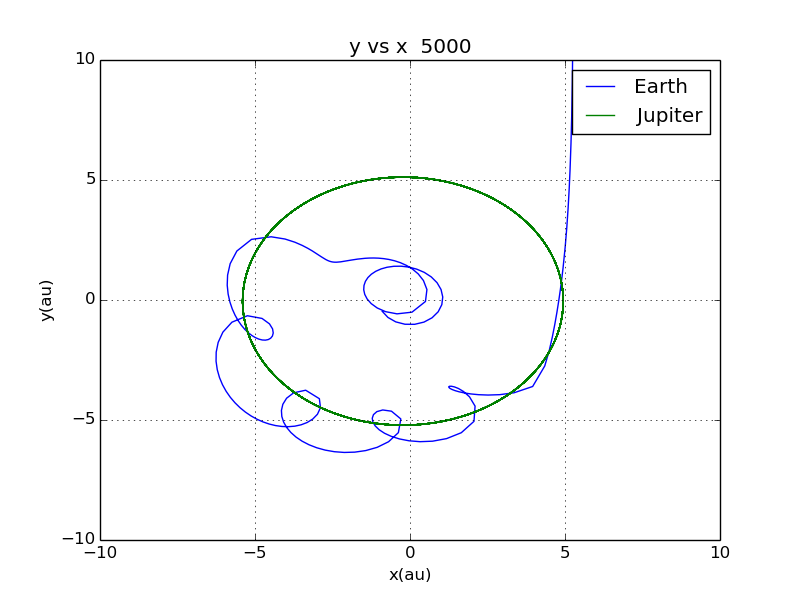
\includegraphics[width=70mm]{EJ_E3V.png}
    \caption{Jupiter with 1000 the original mass} 
    \label{fig7:c} 
    \vspace{4ex}
\end{subfigure}%%
\caption{This shows the position of the Earth and Jupiter with different mass values for Jupiter. From this (a) and (b) we see that that the mass of Jupiter alters Earth's orbit very little. This was done using the Verlet method at n=5000 since the RK4 was very unstable.}
\end{figure}

%**********************************************************************************
% Energy of various configuration of mass of Jupiter
%**********************************************************************************

	With the addition of Jupiter we see that Earth's obit is only slightly perturbed. However as we increase the mass of Jupiter to ten times the original we start seeing a more noticeable deviation. It is until Jupiter's mass is increase by one thousand where we see the Earth's obit is not stable anymore. This causes the Earth to get thrown out of the system. One additional thing to note is that the RK4 for this was very unstable and this can be seen in the values of the total energies.

\begin{figure}[H]
\begin{subfigure}[b]{0.5\linewidth}
    \centering
    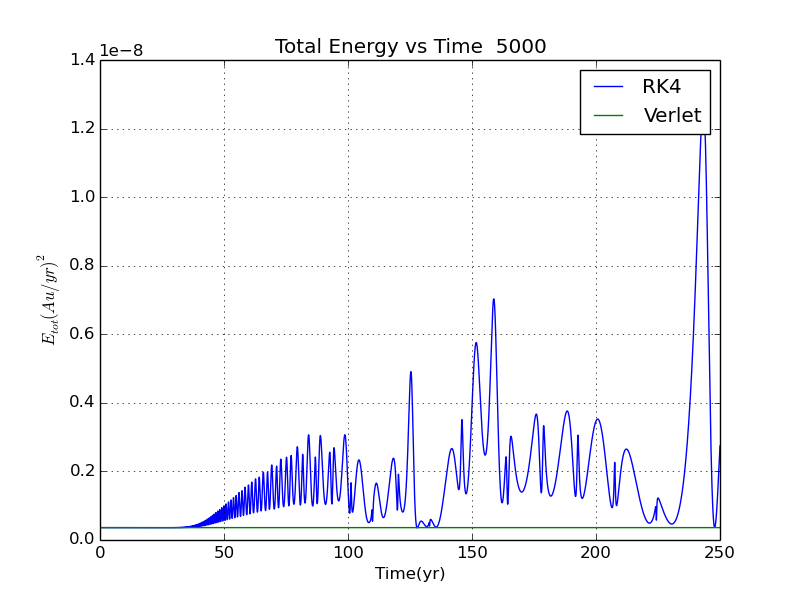
\includegraphics[width=70mm]{Energy_EJ.png}
    \caption{original mass } 
    \label{fig7:a} 
    \vspace{4ex}
\end{subfigure}%%
\begin{subfigure}[b]{0.5\linewidth}
    \centering
    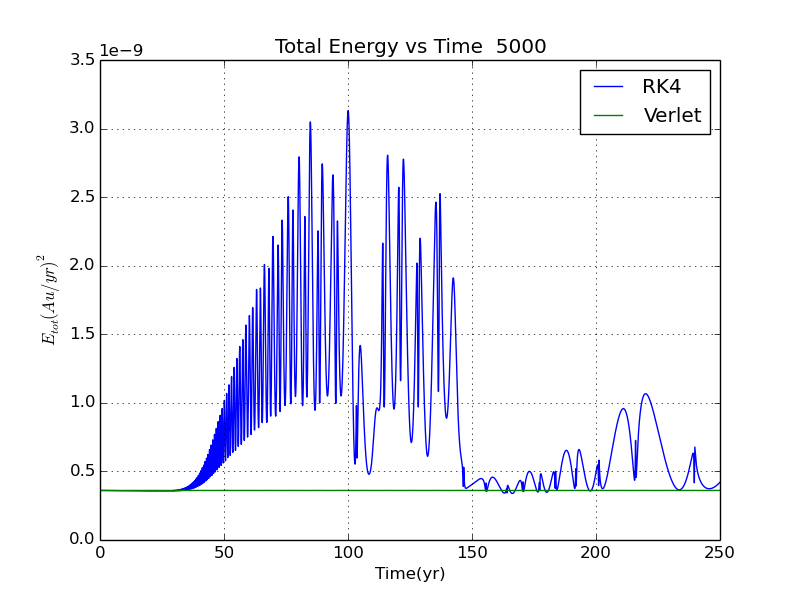
\includegraphics[width=70mm]{Energy_EJ10.png}
    \caption{10 times the original mass} 
    \label{fig7:b} 
    \vspace{4ex}
\end{subfigure}
\begin{subfigure}[b]{0.5\linewidth}
    \centering
    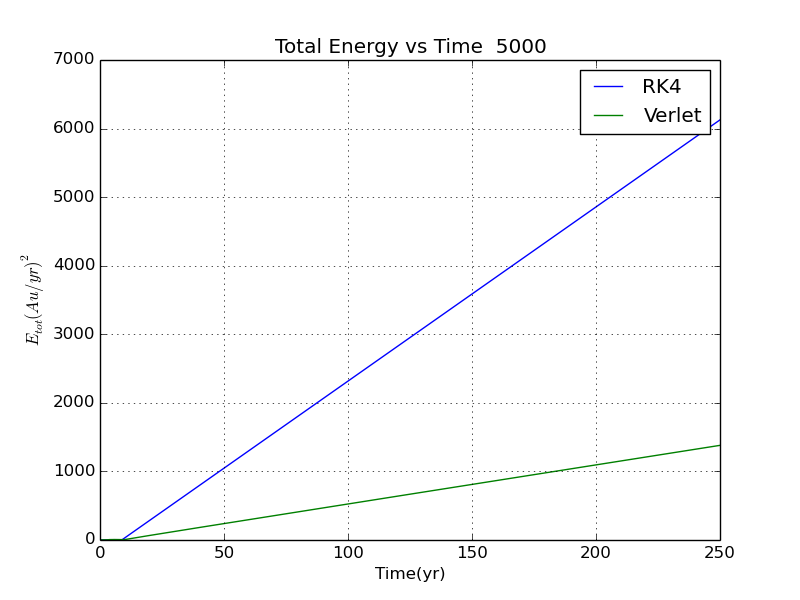
\includegraphics[width=70mm]{EJ_EnergyE3.png}
    \caption{1000 times the original mass} 
    \label{fig7:c} 
    \vspace{4ex}
\end{subfigure}%%
\caption{This shows the total energy for the Earth with different values of the mass of Jupiter. From this we can see that the RK4 method is very unstable and was not used to make plots of the positions. 5000 grid point were used to get the energies.}
\end{figure}





\subsection{Solar System}

	Here I include all of the planets and Pluto. From Figure 7 we see that the inner planets are perturbed more than the outer ones. 
\begin{figure}[H]
\begin{subfigure}[b]{0.5\linewidth}
    \centering
    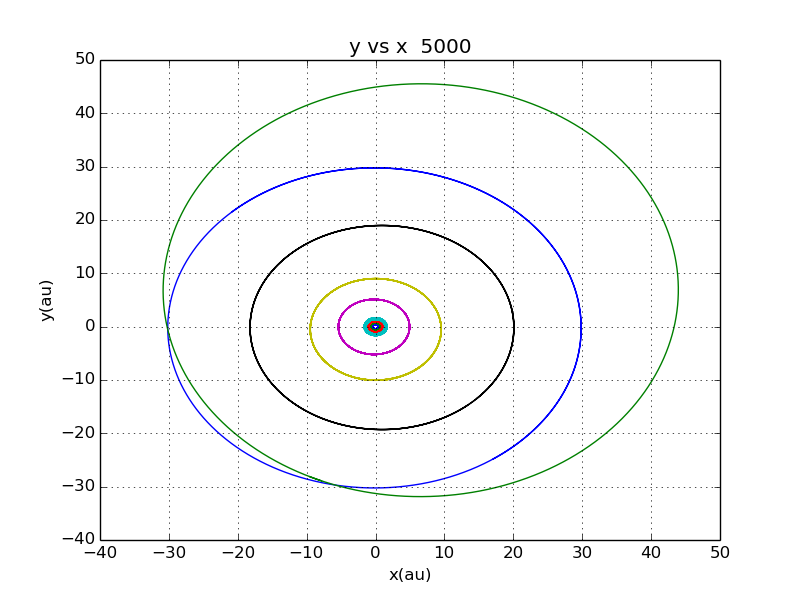
\includegraphics[width=70mm]{Solar.png}
    \caption{Full Solar System} 
    \label{fig7:a} 
    \vspace{4ex}
\end{subfigure}%%
\begin{subfigure}[b]{0.5\linewidth}
    \centering
    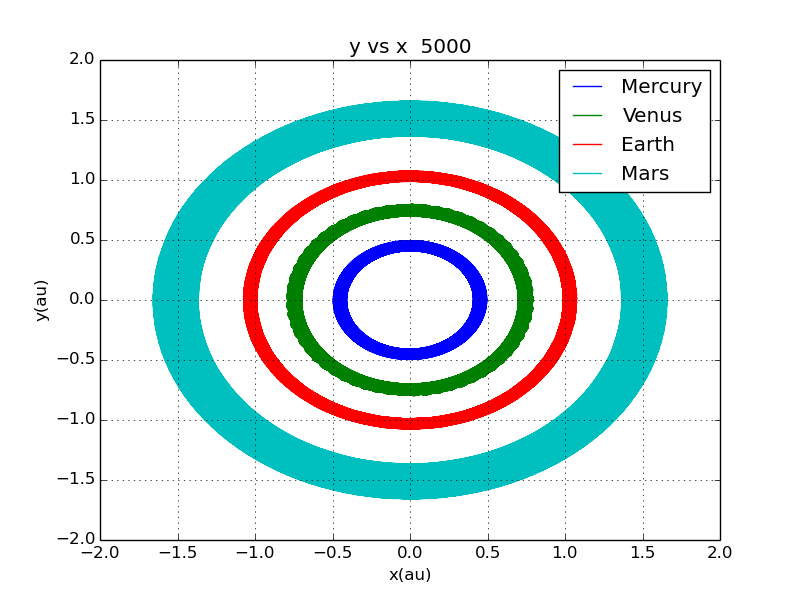
\includegraphics[width=70mm]{Solar_inner.png}
    \caption{Inner Solar System} 
    \label{fig7:b} 
    \vspace{4ex}
\end{subfigure}
\begin{subfigure}[b]{0.5\linewidth}
    \centering
    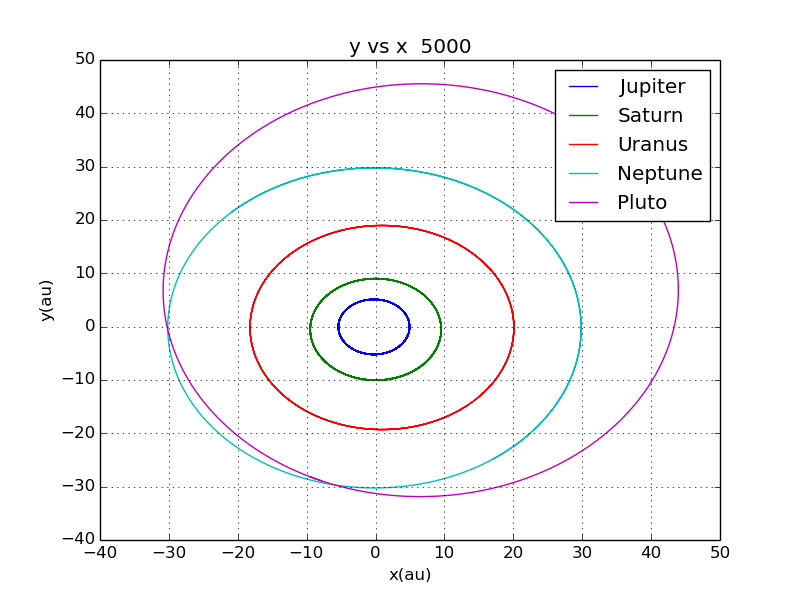
\includegraphics[width=70mm]{Solar_outer.png}
    \caption{Outer Solar System} 
    \label{fig7:c} 
    \vspace{4ex}
\end{subfigure}%%
\caption{This shows the plane view of the orbits of all the planets and Pluto. To see what's really going on I included a view of the inner and outer solar system.}
\end{figure}



%*****************************************************************************************************************************
%This is the Conclusion
%*****************************************************************************************************************************

\section{Conclusion}

	In setting up the equations of motion of the planets with the RK4 and Velocity Verlet(VV) method I conclude that the VV method is a better choice to solve this problem. The results show that the RK4 method is varying more compared to VV. This was expected though since the propagating error in VV is $\ h^4$ and for the RK4 is $\ h^3$. We also found that the velocity needed for circular orbit and also escape the solar system. This are given by $\ 2*\pi$ and $\ 2*\sqrt{2}\pi$ respectively. When adding Jupiter we found that it has only small perturbation on Earth's orbit and this prompted us to hold the Sun in place when the we model all the planets. 

\section{References}
[1] M. Hjorth-Jensen.~Computational Physics, Lecture Notes Spring 2016.\break
[2] Solar System Dynamics. Jet Propulsion Laboratory: California Institute of Technology[accessed May 8 2016; ssd.jpl.nasa.gov/horizons.cgi]

\section{Code Attachment}
\lstinputlisting[language =C++,caption=This sets up the class for planets.]{"/home/quetzalcoatl/Computational_Physics_work/Project3/Code/planet.h"}
\lstinputlisting[language =C++,caption=This gives commands for the class planets.]{"/home/quetzalcoatl/Computational_Physics_work/Project3/Code/planet.cpp"}
\lstinputlisting[language =C++,caption=This sets up the class for the solver system which include the Velocity Verlet and RK4.]{"/home/quetzalcoatl/Computational_Physics_work/Project3/Code/solver.h"}
\lstinputlisting[language =C++,caption=This gives commands for the solver system.]{"/home/quetzalcoatl/Computational_Physics_work/Project3/Code/solver.cpp"}
\lstinputlisting[language =C++,caption=Carries out the Calculation using all the classes set up before.]{"/home/quetzalcoatl/Computational_Physics_work/Project3/Code/Project3.cpp"}

\end{document}

